\section{Diseño del controlador}

\subsection{Control por realimentación de estados}

Gracias al observador de Luenberger desarrollado en la Sección~\ref{sec:obs}, se tiene acceso a estimaciones de rápida convergencia y bajo ruido de todas las variables de estado del sistema. Esto permite realizar un control por realimentación de estados, es decir, diseñar un controlador que cumpla con la siguiente relación de control
\begin{equation*}
    u_k = K \widehat{\mathbf{x}_k},
\end{equation*}
donde $K$ es una matriz de, en nuestro caso particular, $1\times4$. La misma se determina por \emph{pole placement}, utilizando un procedimiento similar al de los polos del observador.

\subsubsection{Diseño del controlador}

En un principio, el control se realizará con el único objetivo de estabilizar al sistema alrededor del punto de equilibrio. Es decir, no habrá una referencia.

Si se utilizaran los estados reales ($\mathbf{x}_k$) en lugar de los observados ($\widehat{\mathbf{x}_k}$), se tendrá
\begin{equation*}
    \mathbf{x}_{k+1} = (A_d + B_d K) \mathbf{x}_k,
\end{equation*}
por lo que ajustar $K$ permite colocar los polos del controlador en el lugar deseado, para conseguir una respuesta temporal acorde. Puede demostrarse que el reemplazo del vector $\mathbf{x}_k$ por su versión observada no mueve los polos del controlador, sino que agrega a la dinámica las singularidades pertenecientes al observador. Si se eligen éstas más rápidas, la respuesta del sistema a lazo cerrado estará aún dominada por los polos del controlador.

Para la elección de los polos del controlador, inicialmente se tomaron de forma tal que sean más lentos que los del observador, para que el control se base en estimaciones precisas de las variables de estado. En particular, se eligieron los polos continuos la mitad de lentos que los polos del observador. Dado que estos polos iniciales resultaron en un control vibrante, se decidió reducir por prueba y error los polos que involucran a las derivadas de las variables medidas, lo que se traduce en una menor dependencia de la acción de control a las variables ruidosas.

Los polos discretos del control por realimentación quedaron en
\begin{align*}
    p_1^{(C,d)} = 0.8040 + 0.1039j &&
    p_2^{(C,d)} = 0.9710 + 0.0470j \\
    p_3^{(C,d)} = 0.8040 - 0.1039j &&
    p_4^{(C,d)} = 0.9710 - 0.0470j.
\end{align*}
Los mismos equivalen a polos continuos en
\begin{align*}
    p_1^{(C,c)} = -10.4955 + 6.4285j &&
    p_2^{(C,c)} = -1.4117 + 2.4172j \\
    p_3^{(C,c)} = -10.4955 - 6.4285j &&
    p_4^{(C,c)} = -1.4117 - 2.4172j.
\end{align*}

La matriz de realimentación $K$ fue calculada por \emph{pole placement}. El resultado obtenido fue
\begin{align*}
    K = \begin{bmatrix}
        0.2533 && -0.0121 && -116.5175 && -30
    \end{bmatrix}.
\end{align*}

\subsubsection{Verificación}

Para la verificación del correcto funcionamiento del controlador, se simuló la respuesta a condiciones iniciales no nulas en la posición del carrito, midiendo todas las variables de estado del sistema\footnotemark{}. El resultado se comparó con la respuesta simulada, y se muestra en la Figura~\ref{fig:noff-vars}.

\footnotetext{Se decidió no realizar un experimento de perturbación tipo impulso golpeando el carrito dado que se dificultó la simulación correcta del mismo para realizar la comparación. Se considera que la respuesta a condiciones iniciales sigue representando correctamente la respuesta natural del lazo cerrado, con una dificultad menor.}

La Figura~\ref{fig:noff-theta} muestra el ángulo de la barra que se obtiene por simulación y que se estima utilizando el observador, para una condición inicial de posición de \qty{0.15}{\m} (y el resto de las variables inicialmente nulas). Vemos que el comportamiento simulado y observado son similares inicalmente, aunque hay un desfasaje de ángulo en estado estacionario que se debe al intento del controlador de reducir el error en estado estacionario.

La Figura~\ref{fig:noff-pos} muestra la posición del carrito simulada y observada. El comportamiento del sistema a lazo cerrado presenta un ligero sobrepico, más marcado en el caso de la posición real, y además tiene un error no nulo en estado estacionario en el caso real debido a la fricción.

Las velocidades angular y lineal se muestran en las Figuras~\ref{fig:noff-omega} y~\ref{fig:noff-vel}. Los comportamientos estimado y simulado son cualitativamente similares. Se nota que la velocidad del carrito estimada tiene un valor no nulo al inicio debido a que el observador espera una posición inicial nula e intenta corregir con la medición de la condición inicial.

\begin{figure}[!htbp]
    \centering
    \begin{subfigure}{0.49\linewidth}
        \centering
        \includegraphics[width=\linewidth]{noff-theta.eps}
        \caption{Ángulo de la barra.}
        \label{fig:noff-theta}
    \end{subfigure}
    \begin{subfigure}{0.49\linewidth}
        \centering
        \includegraphics[width=\linewidth]{noff-pos.eps}
        \caption{Posición del carrito.}
        \label{fig:noff-pos}
    \end{subfigure}

    \begin{subfigure}{0.49\linewidth}
        \centering
        \includegraphics[width=\linewidth]{noff-omega.eps}
        \caption{Velocidad angular de la barra.}
        \label{fig:noff-omega}
    \end{subfigure}
    \begin{subfigure}{0.49\linewidth}
        \centering
        \includegraphics[width=\linewidth]{noff-vel.eps}
        \caption{Velocidad del carrito.}
        \label{fig:noff-vel}
    \end{subfigure}
    \caption{Estados simulados y estimados por el observador para la realimentación de estados.}
    \label{fig:noff-vars}
\end{figure}

\subsection{Agregado de ganancia de \emph{feed-forward}}

\subsubsection{Actualización de observador}

Se optó por ralentizar los polos del observador tras observar un alto nivel de ruido durante el agregado de la matriz de \emph{feed-forward}. La razón de esto fue que la acción de control era muy ruidosa y oscilante en esta instancia y al modificar los polos deseados de todas las formas posibles y no obtener respuesta positiva la única opción restante era que el observador se encontraba siguiendo a la planta demasiado rápido. Se comprobó esto al estudiar más en profundidad su comportamiento, observado previamente en la Figura~\ref{fig:obs-vars}, que ya se preveía que observaba muy rápidamente.

Se requería que el observador siga de manera mucho más suave a las variables, por lo que se partió de la base de disminuir la magnitud de los polos continuos deseados. En principio se fijaron en un valor levemente mayor al polo más rápido de la planta: los cuatro polos deseados rondando los $\SI{-12}{\radian\per\second}$ cuando el polo máximo es $\SI{11.7303}{\radian\per\second}$. Luego se ajustaron finamente los valores hasta obtener señales suaves como las observadas en la \autoref{fig:obs-vars-new}. 

Los polos discretos utilizados finalmente son:
\begin{align*}
	p_1^{(o,d)} = 0.7900 &&
	p_2^{(o,d)} = 0.7867 &&
	p_3^{(o,d)} = 0.7851 &&
	p_4^{(o,d)} = 0.7831.
\end{align*}
Y la matriz de realimentación $L$ resultó en:
\begin{align*}
	L = \begin{bmatrix}
		 0.0003 & 0.0002\\
		-0.4655 & -0.0020\\
		0.0001 & 0.3918\\
		-0.0019 & 1.5908
	\end{bmatrix}.
\end{align*}

\begin{figure}[!htbp]
	\centering
	\begin{subfigure}{0.49\linewidth}
		\centering
		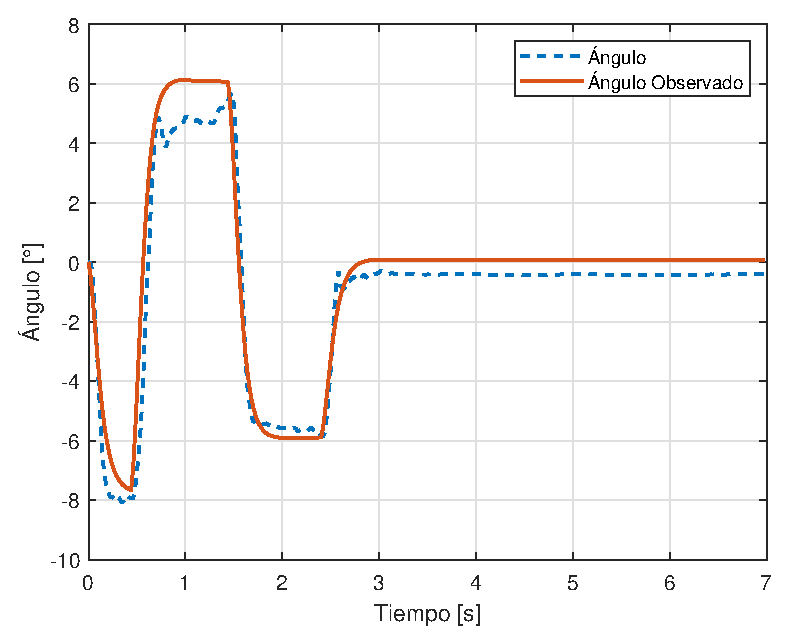
\includegraphics[width=\linewidth]{obs-theta-new.eps}
		\caption{Ángulo de la barra.}
		\label{fig:obs-theta-new}
	\end{subfigure}
	\begin{subfigure}{0.49\linewidth}
		\centering
		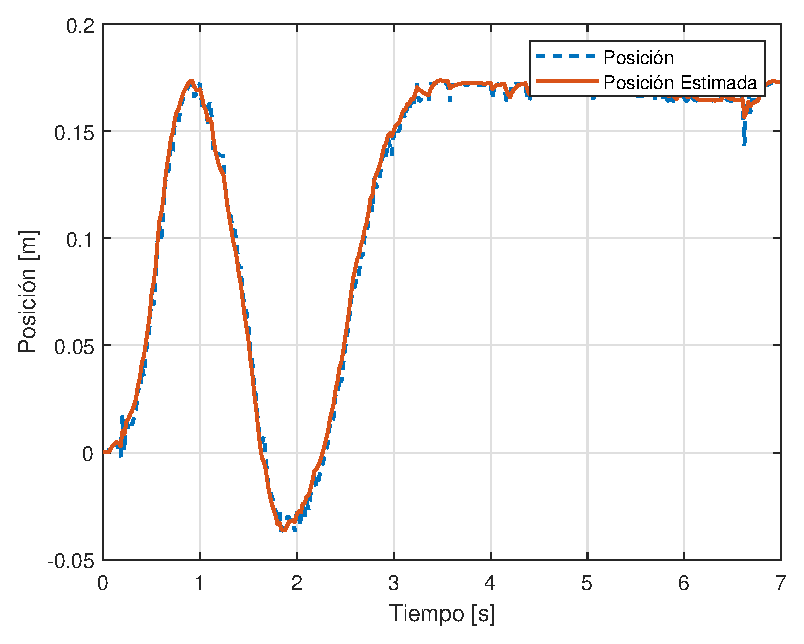
\includegraphics[width=\linewidth]{obs-pos-new.eps}
		\caption{Posición del carrito.}
		\label{fig:obs-pos-new}
	\end{subfigure}
	
	\begin{subfigure}{0.49\linewidth}
		\centering
		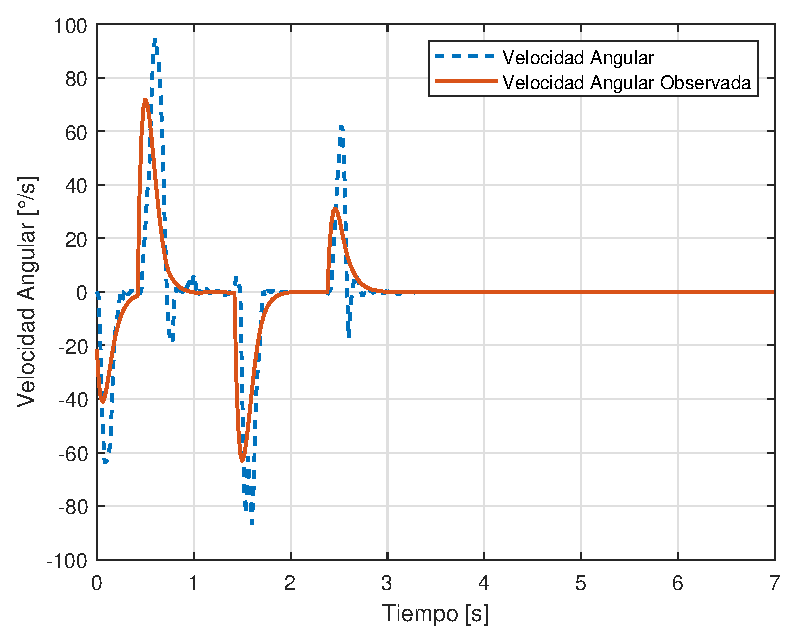
\includegraphics[width=\linewidth]{obs-omega-new.eps}
		\caption{Velocidad angular de la barra.}
		\label{fig:obs-omega-new}
	\end{subfigure}
	\begin{subfigure}{0.49\linewidth}
		\centering
		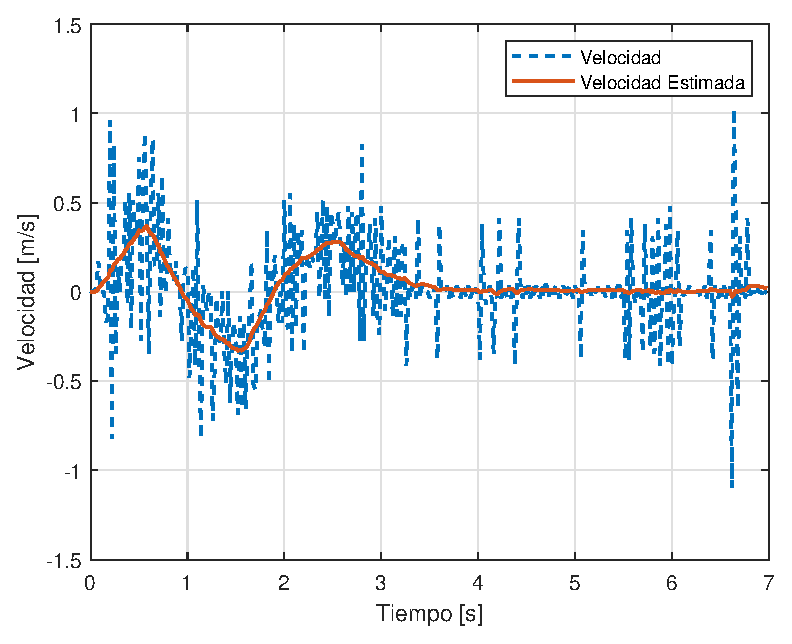
\includegraphics[width=\linewidth]{obs-vel-new.eps}
		\caption{Velocidad del carrito.}
		\label{fig:obs-vel-new}
	\end{subfigure}
	\caption{Estados medidos y estimados por el observador actualizado.}
	\label{fig:obs-vars-new}
\end{figure}

\subsubsection{Cálculo de la matriz}

Para que el sistema a lazo cerrado pueda seguir referencias, se debe agregar un bloque multiplicador por una matriz de \emph{feed-forward} $F$. La misma multiplica a la referencia, que se suma con la realimentación de estados para producir una acción de control. El nuevo sistema queda definido por
\begin{equation*}
    \mathbf{x}_{k+1} = (A_d + B_d K) \mathbf{x}_k + B F r,
\end{equation*}
donde $r$ es la referencia, y $F$ se calcula según
\begin{equation}
    \label{eq:feedforward}
    F = (C_d ( \mathbf{I} - (A_d + B_d K) )^{-1} B_d )^{-1}.
\end{equation}

Las referencias a seguir serán simultáneamente de ángulo $\theta$ y posición $p$. Utilizando los valores de $K$ del diseño anterior, se obtiene
\begin{equation*}
    F = \begin{bmatrix}0 & 116.5175 \end{bmatrix}.
\end{equation*}
Notar que la última inversa a calcular en \eqref{eq:feedforward} es en realidad una pseudoinversa de una matriz rectangular, por lo que el controlador no será capaz de controlar en función de ambas referencias en forma simultánea. Esto es esperable, ya que no hay manera de mover el carrito para lograr establecer la referencia de posición sin realizar ningún movimiento de la barra.

\subsubsection{Verificación}

Para verificar el correcto funcionamiento del controlador, se simularon referencias tipo escalón de posición, con $\theta_{\mathrm{ref}}=0$. Se midieron las respuestas temporales de todas las variables de estado utilizando el observador, y se compararon con simulaciones, como se observa en la Figura~\ref{fig:ff-vars}.

\begin{figure}[!htbp]
    \centering
    \begin{subfigure}{0.49\linewidth}
        \centering
        \includegraphics[width=\linewidth]{ff-theta.eps}
        \caption{Ángulo de la barra.}
        \label{fig:ff-theta}
    \end{subfigure}
    \begin{subfigure}{0.49\linewidth}
        \centering
        \includegraphics[width=\linewidth]{ff-pos.eps}
        \caption{Posición del carrito.}
        \label{fig:ff-pos}
    \end{subfigure}

    \begin{subfigure}{0.49\linewidth}
        \centering
        \includegraphics[width=\linewidth]{ff-omega.eps}
        \caption{Velocidad angular de la barra.}
        \label{fig:ff-omega}
    \end{subfigure}
    \begin{subfigure}{0.49\linewidth}
        \centering
        \includegraphics[width=\linewidth]{ff-vel.eps}
        \caption{Velocidad del carrito.}
        \label{fig:ff-vel}
    \end{subfigure}
    \caption{Estados simulados y estimados por el observador para la realimentación de estados con \emph{feed-forward}.}
    \label{fig:ff-vars}
\end{figure}

La posición del carrito se observa en la Figura~\ref{fig:ff-pos}. Vemos que debido a la fricción, la posición real del carrito presenta un error en estado estacionario bastante grande, en particular para el segundo escalón de referencia. Sin embargo, el comportamiento cualitativo del sistema real es similar al simulado, y se observa un seguimiento a las referencias.

La Figura~\ref{fig:ff-theta} muestra el ángulo de la barra. Vemos que no se mantiene en cero grados como la referencia impuesta, debido a que no pueden seguirse ambas referencias simultáneamente. El comportamiento cualitativo es similar entre simulación y realidad.

Las Figuras~\ref{fig:ff-omega} y~\ref{fig:ff-vel} muestran las velocidades angular y del carrito, simuladas y estimadas. Vemos que hay una buena concordancia entre simulación y realidad.

\subsection{Acción integral}

Con el fin de eliminar el error en estado estacionario que inevitablemente ocurre por efecto de la fricción, se agrega acción integral al controlador. En este paso también se buscará un control rápido, cuyo tiempo de establecimiento sea menor a \qty{2.5}{\s} y tenga un sobrepico menor al \qty{15}{\percent}.

Para ello, se vuelve a cerrar el lazo con un nuevo controlador integral, regido por la ecuación
\begin{equation*}
    q_{k+1} = q_k + T_s e_k,
\end{equation*}
donde $e_k = r_k - p_k$, notando que ahora la planta tiene una única salida (la posición $p$) y una única referencia de posición ($r$). Ahora se tiene \[C_d = [ 0 \; 0 \; 1 \; 0 ]. \]

El sistema completo queda regido por
\begin{align*}
    \begin{bmatrix}\mathbf{x}_{k+1} \\ q_{k+1} \end{bmatrix} &=
        \left( A_{\mathrm{ext}} + B_{\mathrm{ext}} \begin{bmatrix}K & H\end{bmatrix} \right)
        \begin{bmatrix}\mathbf{x}_{k} \\ q_k \end{bmatrix},
\end{align*}
donde
\begin{align*}
    A_{\mathrm{ext}} = \begin{bmatrix} A_{d} & 0 \\ -C_{d} T_s & \mathbf{I} \end{bmatrix}
        && B_{\mathrm{ext}} = \begin{bmatrix}B_d \\ 0\end{bmatrix}.
\end{align*}

\subsubsection{Diseño}

Los polos elegidos para el control fueron los siguientes
\begin{align*}
	p_1^{(C,c)} = -7 &&
	p_2^{(C,c)} = -2.7 &&
	p_3^{(C,c)} = -8 &&
    p_4^{(C,c)} = -2.7 &&
    p_5^{(C,c)} = -3.
\end{align*}
En discreto, se corresponden con
\begin{align*}
   p_1^{(C,d)} = 0.8694 &&
   p_2^{(C,d)} = 0.9474 &&
   p_3^{(C,d)} = 0.8521 &&
   p_4^{(C,d)} = 0.9474 &&
   p_5^{(C,d)} = 0.9418.
\end{align*}

La matriz de realimentación $K$, calculada por \emph{pole-placement}, resultó en
\begin{align*}
    K = \begin{bmatrix}
        0.20602 &  -0.019697 &  -168.14 & -57.641
    \end{bmatrix}.
\end{align*}
El coeficiente asociado al control integral resultó en $H = 120.73$.

\subsubsection{Verificación}

Para la verificación del funcionamiento del controlador con acción integral, se introdujo una sucesión de referencias tipo escalón, y se midieron las variables de estado observadas. El resultado fue comparado con una simulación, y los resultados se muestran en la Figura~\ref{fig:int-vars}.

\begin{figure}[!htbp]
	\centering
	\begin{subfigure}{0.49\linewidth}
		\centering
		\includegraphics[width=\linewidth]{int-theta.eps}
		\caption{Ángulo de la barra.}
		\label{fig:int-theta}
	\end{subfigure}
	\begin{subfigure}{0.49\linewidth}
		\centering
		\includegraphics[width=\linewidth]{int-pos.eps}
		\caption{Posición del carrito.}
		\label{fig:int-pos}
	\end{subfigure}
	
	\begin{subfigure}{0.49\linewidth}
		\centering
		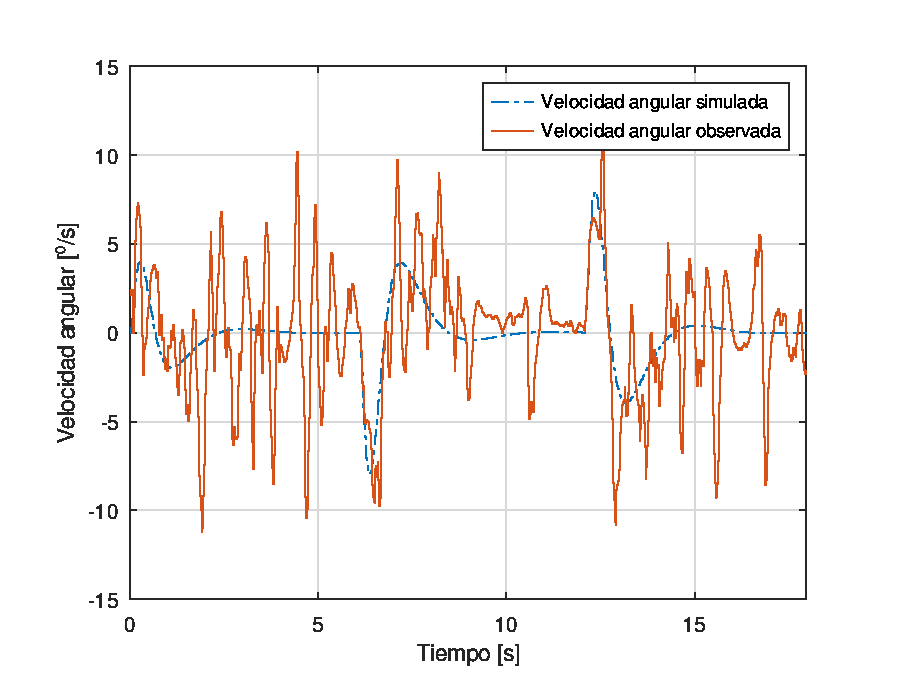
\includegraphics[width=\linewidth]{int-omega.eps}
		\caption{Velocidad angular de la barra.}
		\label{fig:int-omega}
	\end{subfigure}
	\begin{subfigure}{0.49\linewidth}
		\centering
		\includegraphics[width=\linewidth]{int-vel.eps}
		\caption{Velocidad del carrito.}
		\label{fig:int-vel}
	\end{subfigure}
	\caption{Estados medidos y estimados por el observador, para el controlador con acción integral.}
	\label{fig:int-vars}
\end{figure}

La posición del carrito simulada y estimada por el observador se muestra en la Figura~\ref{fig:int-pos}. Se observa que se tiene un tiempo de establecimiento del orden de los \qty{2}{\s}, menor a los \qty{2.5}{\s} máximos especificados. En cuanto al sobrepico, no se alcanza el objetivo del \qty{15}{\percent} en teoría, pero la fricción no modelada logra detener el carro, haciendo que no haya sobrepico alguno y sí se cumpla con el requerimiento en la planta real.

Debido al efecto de la fricción, se observa cierto error en estado estacionario, el cual no es excesivamente grande. Además, la presencia de acción integral permite continuar aumentando la acción de control con el objetivo de reducir dicho error.

La Figura~\ref{fig:int-theta} muestra el ángulo simulado y estimado por el observador. Hay una buena concordancia entre simulación y realidad. La misma figura muestra además la acción de control enviada al servomotor. Debido a la presencia de acción integral, siempre está presente el riesgo de saturar el actuador. Sin embargo, se verifica que para estos experimentos la acción de control no supera los \qty{15}{\degree} en valor aboluto, lo que deja un margen muy amplio respecto de los límites impuestos de \qty{30}{\degree}.

La velocidad angular simulada y estimada por el observador se muestra en la Figura~\ref{fig:int-omega}. Vemos que la observación de la velocidad angular se ve muy afectada por el ruido, al menos en una proporción mayor que durante lops experimentos sin acción integral que utilizaban el mismo observador.

La velocidad del carrito, cuya simulación y estimación se muestran en la Figura~\ref{fig:int-vel}, muestran un nivel de ruido inferior al de la velocidad angular, y un relativamente buen seguimiento.

La razón del aumento en el ruido parece deberse a los mayores valores de ganancia utilizados en la realimentación, especialmente las entradas 3 y 4 de la matriz $K$, las cuales son entre un \qty{40}{\percent} y el doble de grandes que las usadas para los primeros controladores. Esto produce acciones de control más agresivas, lo que introduce cierto ruido. Además, ese ruido se traduce en errores de medición, lo que afecta la acción de control en un círculo vicioso. Aún así, como el comportamiento del controlador es satisfactorio en términos del tiempo de establecimiento, y no presenta \emph{overshoot}, se decidió tolerar estos efectos.

% vim: ts=4 sts=4 sw=4 et lbr
